\documentclass[../cours_3e.tex]{subfiles}
\begin{document}
\setcounter{chapter}{10}
\chapter{Hasard et probabilités}
\label{ch:probabilites}
\begin{objectif}
Décrire une expérience, compter les issues, calculer des probabilités sur une ou deux épreuves et interpréter une simulation. Prérequis : fractions et fréquences.
\end{objectif}
\section{Vocabulaire du hasard}
\begin{definition}
Une \textbf{expérience aléatoire} a un résultat incertain avant sa réalisation. Une \textbf{issue} est un résultat possible. L'\textbf{univers} est l'ensemble des issues. Un \textbf{événement} est un ensemble d'issues.
\end{definition}
Pour le lancer d'un dé à six faces, l'univers est $\{1,2,3,4,5,6\}$. L'événement « obtenir un nombre pair » est $\{2,4,6\}$. « Obtenir $8$ » est impossible ; « obtenir moins de $7$ » est certain.
\begin{definition}
Une probabilité attribue des nombres positifs ou nuls aux issues, de somme $1$. La probabilité d'un événement est la somme des probabilités de ses issues.
\end{definition}
On note $P(A)$ la probabilité de l'événement $A$. Il en découle $0\leq P(A)\leq1$, $P(\text{impossible})=0$ et $P(\text{certain})=1$.
\begin{attention}
Le modèle doit être précisé. Un dé « équilibré » a des faces de même probabilité ; on ne peut pas supposer cette égalité pour un dé truqué.
\end{attention}
\section{Équiprobabilité et dénombrement}
\begin{definition}
Il y a \textbf{équiprobabilité} lorsque toutes les issues ont la même probabilité.
\end{definition}
\begin{propriete}
Dans un univers fini équiprobable à $N$ issues,
\[P(A)=\frac{\text{nombre d'issues favorables à }A}{N}.\]
\end{propriete}
\begin{demonstration}
Si chaque issue a une probabilité $p$, leur somme vaut $Np=1$, donc $p=1/N$. Pour $m$ issues favorables, la somme vaut $m/N$.
\end{demonstration}
Pour un dé équilibré, $P(\text{pair})=3/6=1/2=0{,}5=50\,\%$.
Une urne contient $2$ boules rouges et $1$ bleue, toutes indiscernables au toucher. Les \emph{boules} sont équiprobables, les \emph{couleurs} ne le sont pas : $P(R)=2/3$ et $P(B)=1/3$.
\section{Événement contraire et réunions}
\begin{definition}
L'événement contraire $\overline A$ contient les issues qui ne sont pas dans $A$. Deux événements sont incompatibles lorsqu'ils n'ont aucune issue commune.
\end{definition}
\begin{propriete}
\[P(\overline A)=1-P(A).\]
Si $A$ et $B$ sont incompatibles, $P(A\text{ ou }B)=P(A)+P(B)$.
\end{propriete}
\begin{demonstration}
$A$ et son contraire partagent tout l'univers sans recouvrement. Leurs probabilités s'ajoutent donc à $1$. Pour deux événements incompatibles, l'addition ne compte aucune issue deux fois.
\end{demonstration}
\approfondissement S'ils ne sont pas incompatibles, il faut retirer le double comptage :
\[P(A\text{ ou }B)=P(A)+P(B)-P(A\text{ et }B).\]
Sur un dé, « pair ou supérieur à $4$ » donne $\{2,4,5,6\}$ : $3/6+2/6-1/6=4/6$, car $6$ appartient aux deux événements.
\section{Deux épreuves : représenter toutes les issues}
\begin{exemple}[Deux dés]
On lance deux dés équilibrés indépendants. Une issue est un couple ordonné $(i;j)$. Il y en a $6\times6=36$, équiprobables. Les six couples de somme $7$ sont
\[(1;6),(2;5),(3;4),(4;3),(5;2),(6;1).\]
La probabilité d'une somme $7$ est $6/36=1/6$.
\end{exemple}
\begin{attention}
Les sommes $2,3,\ldots,12$ ne sont pas équiprobables. Il n'existe qu'un couple de somme $2$, contre six de somme $7$. On ne divise donc pas systématiquement par $11$.
\end{attention}
Un tableau à double entrée évite les oublis. Dans une urne de boules $R_1,R_2,B$, deux tirages \textbf{avec remise} donnent :
\[
\begin{array}{c|ccc}
\text{1er}\backslash\text{2e}&R_1&R_2&B\\\hline
R_1&(R_1,R_1)&(R_1,R_2)&(R_1,B)\\
R_2&(R_2,R_1)&(R_2,R_2)&(R_2,B)\\
B&(B,R_1)&(B,R_2)&(B,B)
\end{array}
\]
Les neuf couples sont équiprobables si l'on mélange correctement à chaque tirage. Quatre sont rouge-rouge, donc $P(RR)=4/9$. « Au moins une bleue » est le contraire : $1-4/9=5/9$.
\section{Lire un arbre sans supposer une indépendance}
\begin{center}
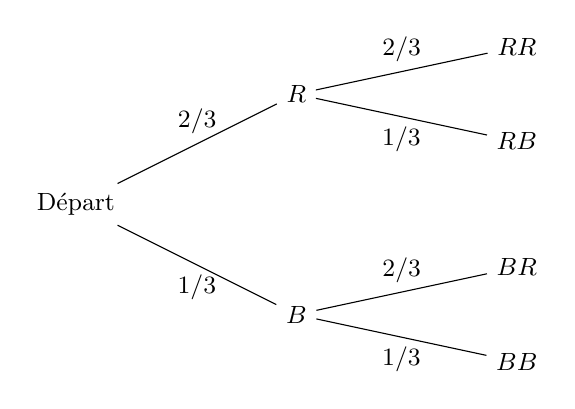
\begin{tikzpicture}[x=2.8cm,y=1cm,every node/.style={font=\small}]
\node (O) at(0,0){Départ};
\node (R) at(1,1.4){$R$};\node (B) at(1,-1.4){$B$};
\node (RR) at(2,2){$RR$};\node (RB) at(2,.8){$RB$};
\node (BR) at(2,-.8){$BR$};\node (BB) at(2,-2){$BB$};
\draw(O)--node[above]{$2/3$}(R);\draw(O)--node[below]{$1/3$}(B);
\draw(R)--node[above]{$2/3$}(RR);\draw(R)--node[below]{$1/3$}(RB);
\draw(B)--node[above]{$2/3$}(BR);\draw(B)--node[below]{$1/3$}(BB);
\end{tikzpicture}
\end{center}
Cet arbre décrit les couleurs avec remise. Le produit $(2/3)(2/3)=4/9$ correspond aux quatre couples rouges du tableau : sur trois premiers choix, deux sont rouges, puis deux seconds choix sur trois le sont.

\textbf{Sans remise}, une boule tirée n'est pas replacée. Il reste deux boules. Les six couples de boules distinctes sont équiprobables ; seuls $(R_1,R_2)$ et $(R_2,R_1)$ sont rouge-rouge, donc $P(RR)=2/6=1/3$. Sur l'arbre, après un rouge, la probabilité d'un deuxième rouge devient $1/2$. Après un bleu, elle vaut $1$. Le second tirage dépend du premier.

\begin{attention}
Ne pas multiplier deux probabilités isolées sans examiner l'expérience. Sur un chemin, le second facteur décrit ce qui est possible \emph{après} le premier résultat. Le dénombrement détaillé est la méthode de référence ici ; le formalisme des probabilités conditionnelles appartient à la suite de la scolarité.
\end{attention}
\section{Fréquences observées et probabilités}
Sur $n$ répétitions, la fréquence observée d'un événement est $F_n=k/n$, où $k$ est le nombre de réalisations. Elle dépend de l'expérience. La probabilité est une valeur du modèle.
\begin{exemple}
Si un dé donne $173$ six sur $1000$ lancers, la fréquence est $0{,}173$. Cela ne prouve pas que le dé est truqué, ni que sa probabilité vaut exactement $0{,}173$.
\end{exemple}
\admis{Sous des répétitions indépendantes dans les mêmes conditions, les fréquences tendent à se rapprocher de la probabilité lorsque le nombre d'essais augmente, dans un sens probabiliste. Ce résultat général n'est pas démontré au collège. Une simulation l'illustre, sans le prouver et sans garantir une amélioration à chaque lancer.}
Après cinq piles avec une pièce équilibrée, la probabilité du prochain pile reste $1/2$ si les lancers sont indépendants. Le hasard n'a pas à « compenser » immédiatement.
\utilite{Évaluer une chance, comparer des jeux et distinguer une fluctuation normale d'une certitude. Les simulations du chapitre 19 relient le calcul théorique à l'observation.}
\begin{retenir}
Définir des issues suffisamment précises, vérifier l'équiprobabilité, puis compter. « Au moins un » se calcule souvent plus facilement par l'événement contraire. Fréquence et probabilité sont liées mais différentes.
\end{retenir}
\end{document}
